\documentclass[UTF8]{ctexart}
\usepackage{graphicx}
\usepackage{cite}
\usepackage{enumerate}
\usepackage{geometry}
\title{EI339 Class Project Report}
\author{孟令佳 516030910553}
\date{2018年12月}
\geometry{a4paper}
\begin{document}
\maketitle
\tableofcontents
\newpage
\section{组员分工}
\begin{enumerate}
    \item 陈子轩 LSTM模型搭建,底层LSTM实现,实验报告撰写
    \item 孟令佳 原始数据处理,DNN模型搭建与调参,LSTM模型搭建与调参,实验报告撰写
\end{enumerate}
\section{工作环境}
\begin{enumerate}
    \item windows 10
    \item python 3.6.7 64bit \{base:conda\}
    \item python module: pytorch, numpy, pandas
\end{enumerate}
\section{问题描述}
\subsection{股价变动机制}
\begin{figure}[!htbp]
\centering
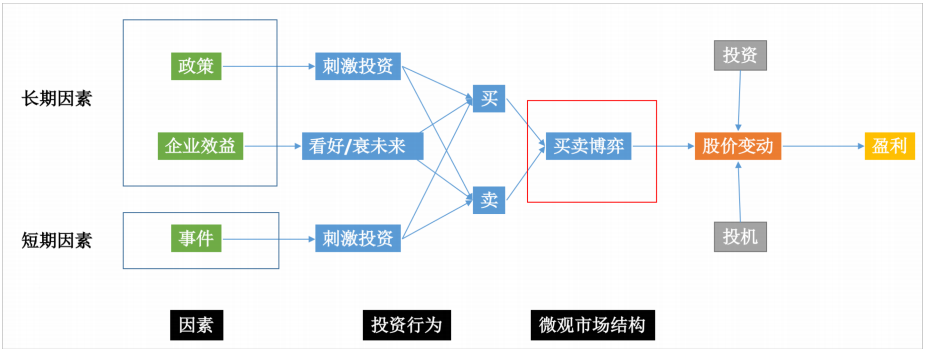
\includegraphics[scale = 0.6]{p1.png}
\caption{股价变动机制}
\end{figure}
如图所示,影响股价变动的机制有长期因素和短期因素,他们都最终归结为买卖博弈来影响价格。买卖博弈可以通过三个方面体现:已公开的买卖需求、正在实施的买卖动作、持币观望。已公开的买卖需求可以通过订单簿来体现,正在实施的买卖动作经研究可以看做是随机尝试的实现,而第三类信息是难以获得的。本次大作业主要研究订单簿对价格的影响。
\subsection{数据描述}
订单簿的数据为:
\begin{enumerate}[*]
    \item 日期(Date)
    \item 时间(Time)
    \item 申买价(Bid Price)
    \item 申买量(Bid Volume)
    \item 申卖价(Ask Price)
    \item 申卖量(Ask Volume)
    \item 最新成交价(Last Price)
    \item 中间价(MidPrice = (Bid Price + Ask Price) / 2)
    \item 当前累计成交数量(Volume)
\end{enumerate}
\subsection{任务要求}
通过对订单簿中数据的学习,预测下20个时间点中间价(mid price)的均值
\section{算法设计}
\subsection{LSTM}
\subsubsection{算法介绍}
LSTM(Long-Short-Term-Memory)是RNN的一种变体,要了解LSTM,首先需要了解RNN的工作原理,如下图
\begin{figure}[!htbp]
\centering
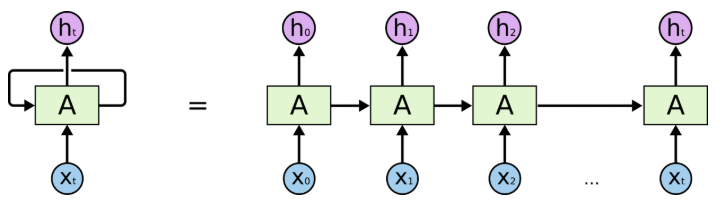
\includegraphics[scale = 0.8]{p3.png}
\caption{Recurrent Neural Network(RNN)\cite{1}}
\end{figure}
\paragraph*{RNN的结构}
传统的RNN包含一个循环态,如图2左边的单元,它可以读入一个输入$x_t$,输出一个$h_t$,从而将状态转移到下一个时间点。如果将这个单元按照时间序列展开则可以得到图二右边的单元序列。由于它的链式的特征,他自然与时间序列和列表产生关联,从而可以解决由于时间的推移所带来的问题。RNN可以利用对先前信息的理解对后续的事件做出预测,例如我们想要预测"the clouds are in the sky"这句话的最后一个单词, 由于根据前面的句子很显然最后一个词就是sky,所以通过RNN可以准确的预测出来。
\paragraph*{RNN的缺陷}
但是如果我们想要预测“I was born in Japan, .... I speak Japanese"这样需要跨越较长的时间序列才能获得的信息时则显得力不从心,在处理较长序列时,RNN会不可避免的产生梯度消失或者梯度爆炸的问题,这是由于RNN自身结构而产生的问题,但是幸运的是, LSTM并不存在这样的问题。
\paragraph*{LSTM的结构}
LSTM在RNN的基础上,改进了工作单元的机构,传统的RNN模块包含的是重复单一的层,但是LSTM的重复模块包含的是四个交互的层。如下图
\begin{figure}[!htbp]
    \centering
    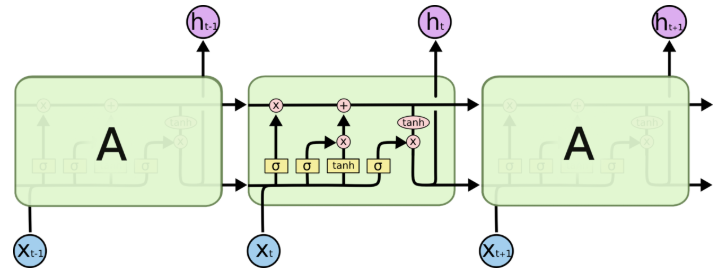
\includegraphics[scale = 0.8]{p4.png}
    \caption{LSTM的重复模块\cite{1}}
\end{figure}
我们将结合图5更进一步介绍LSTM的内部信息。
\begin{figure}[!htbp]
    \centering
    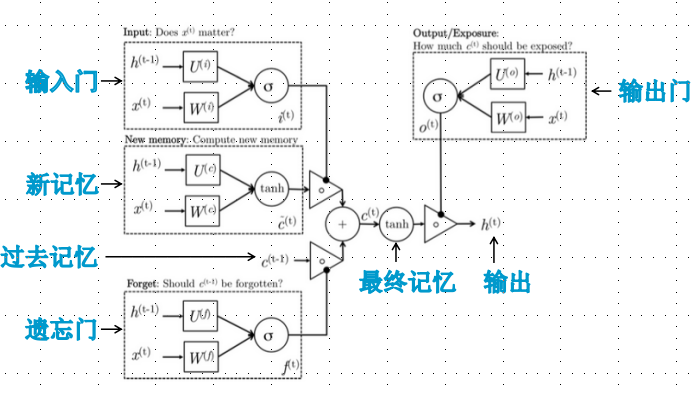
\includegraphics[scale = 0.8]{p5.png}
    \caption{LSTM的内部结构\cite{2}}
\end{figure}
\paragraph*{1. 决定丢弃信息}对于上一个时间点的信息,首先决定丢弃那些信息,这一步通过遗忘门来决定,该门将读取$h_{t-1}$和$x_t$,输出一个$f_t$,$f_t$内的值为$[0,1]$,0表示完全舍弃,1表示完全保留。
$$f_t = \sigma(W_f\cdot x_t + U_f\cdot h_{t-1} + b_f)$$
\paragraph*{2. 确定新信息}
下一步将是决定什么样的新信息将被存放在细胞状态中,这一步包含两个门,输入门和新记忆,\textbf{新记忆}通过tanh函数构建候选信息向量,\textbf{输入门}通过sigmoid函数判定什么值将要更新。
$$i_t = \sigma(W_i\cdot x_t + U_i\cdot h_{t-1} + b_f)$$
$$a_t = \sigma(W_a\cdot x_t + U_a\cdot h_{t-1} + b_f)$$
\paragraph*{3. 更新细胞状态}
然后,新记忆将于旧记忆结合构成新的细胞状态
$$C_t = f_t\cdot C_{t-1} + i_t \cdot a_t$$
\paragraph*{4. 确定新信息}
最后,我们通过一个\textbf{输出门}决定什么将被输出
$$o_t = \sigma(W_o\cdot x_t + U_o\cdot h_{t-1} + b_f)$$
$$h_t = tanh(C_t)\cdot o_t$$
\subsubsection{建模方式}
\begin{figure}[!htbp]
    \centering
    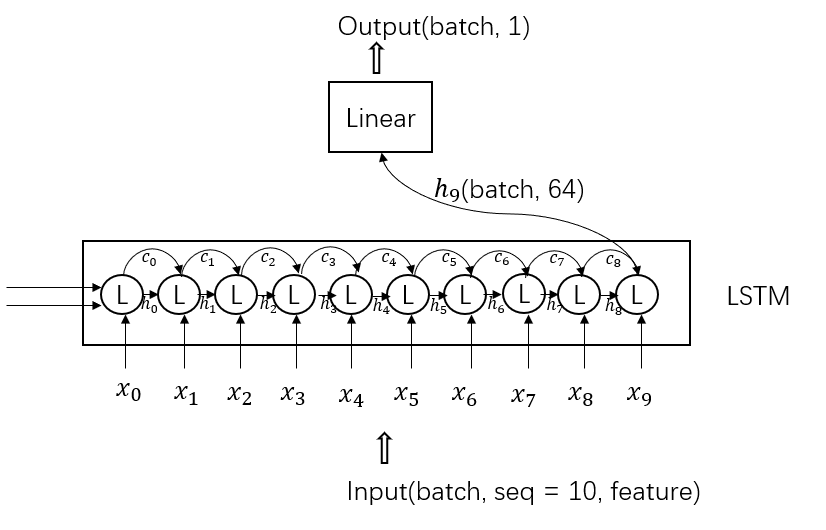
\includegraphics[scale = 0.6]{p6.png}
    \caption{LSTM建模\cite{2}}
\end{figure}
如图5,根据LSTM的模型特征,我们选择通过前10天的订单簿数据预测下20个时间点中间价(mid price)的均值,即时间序列长度seq = 10。选择的输入特征为订单簿的各类数据,包括['MidPrice', 'LastPrice', 'Volume', 'BidPrice1', 'BidVolume1', 'AskPrice1', 'AskVolume1', 'VolDiff'],其中VolDiff由相邻两日的Volume之差组成

\subsection{DNN}
DNN(深度神经网络)可以理解为有很多隐藏层的神经网络(NN)。多层神经网络和深度神经网络DNN其实也是指的一个东西,DNN有时也叫做多层感知机(Multi-Layer perceptron,MLP)
\subsubsection{算法介绍}
DNN的结构其实相对简单,本质上是由很多个感知机组成,第一层为输入层,中间层为隐藏层,最后一层为输出层。结构如图6所示
\begin{figure}[!htbp]
    \centering
    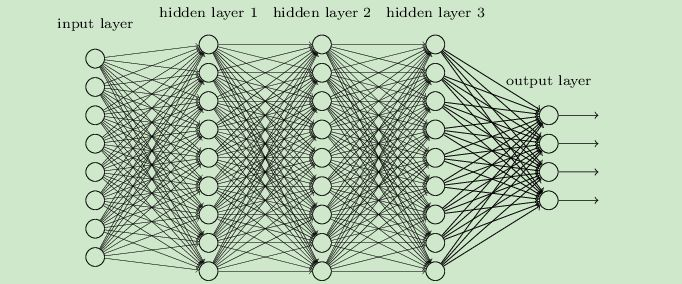
\includegraphics[scale = 0.5]{p10.jpg}
    \caption{DNN结构示意图}
\end{figure}
DNN层与层之间是全连接的,也就是说,第i层的任意一个神经元一定与第i+1层的任意一个神经元相连。虽然DNN看起来很复杂,但是从小的局部模型来说,还是和感知机一样,即一个线性关系 $z = \sum_{}^{}{w_{i} x_{i}}+b$ 加上一个激活函数 $\sigma(z)$

\subsubsection{建模方式}
我们的模型采用了一层输入层,两层隐藏层,一层输出层的四层深度神经网络结构。层与层之间均为全连接层,我们同时采用了线性整流函数(relu)为激活函数。
\subsection{模型搭建与调参}
\paragraph{}我们选择用pytorch进行了模型搭建,参数梯度下降我们采用了Adam算法进行优化。由于DNN的效果并不理想,最终效果只能到0.002左右,我们并没有进行过多的尝试,这里主要对LSTM模型进行说明。对于LSTM的参数我们进行了多种尝试。
\paragraph{}首先对于数据集,我们尝试了不同的$BATCH\_SZIE$ ,但对结果的影响并不大。但是数据的顺序十分重要的,不能够随机打乱。LSTM本身就是一个针对时间序列的模型,因此需要注意数据的有序性。
\paragraph{}标准的LSTM只有一层隐藏层,我们设置增加了LSTM的隐藏层层数为两层,同时增加了一层单独的输出层,将隐藏层的输出映射为一个预测值。
对于隐藏层的层数,隐藏层的大小尝试了多组参数后,我们发现,参数的调整影响并不是很大,只是学习率和学习的epoch数量影响比较大,epoch要足够大以充分利用数据对模型进行训练,相对应的学习率要适当调低,以避免过拟合或者梯度下降过快,导致模型难以收敛。因此我们将epoch设置为了50,学习率设置为了10的负五次方。最后达到public score为0.0153的成绩
\section{数据分析与处理}
数据预处理是非常重要的一步,数据和特征决定了机器学习的上限,而模型和算法只是逼近这个上限而已,数据预处理的常见方式有:归一化,标准化,特征二值化等等.
\subsection{数据归一化}
\paragraph{}归一化方法:标准化,将数据归一化成均值为0,方差为1的数据:
$$x_{norm} = \frac{x - x_{mean}}{x_{std\_error}},\forall x \in Dataset $$

\paragraph{}本次的实验数据由于提供的数据量纲不同,数值范围相差很大,如果不进行预处理,可能会导致梯度下降很慢,进而使模型难以收敛。因此对数据的进行归一化预处理是十分必要的。
\paragraph{}在没有进行归一化操作时,我们进行过模型训练,最终结果也是很难收敛,预测效果也很差,提交后的评分在0.8以上,之后我们尝试数据统一进行归一化,但是结果也不尽如人意,学习的效果也不令人满意。合理的选择归一化的分段也是很重要的
\begin{figure}[!htbp]
    \centering
    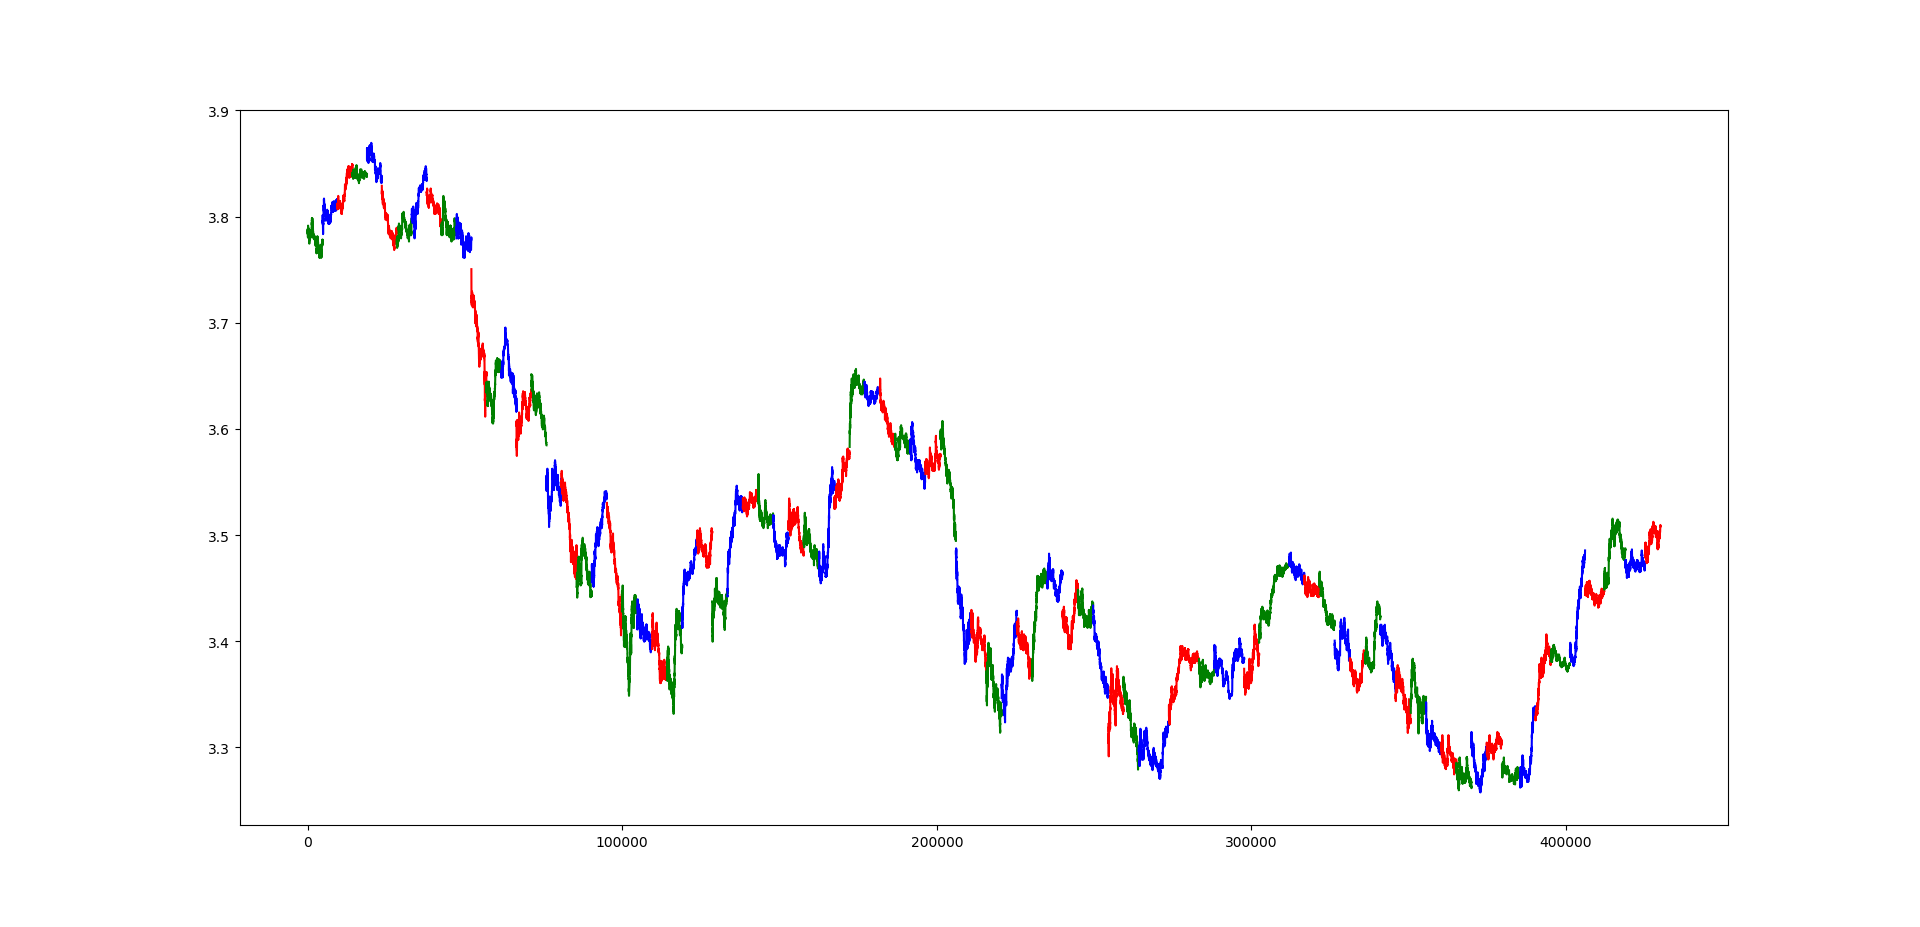
\includegraphics[scale = 0.3]{p8.png}
    \caption{MidPrice变化图(相邻相同颜色是同一天的数据)}
\end{figure}
\paragraph{}图6显示的是训练集MidPrice随时间变化图,可以看到每一天的数据分布虽然都局限某一相对范围内,分布也比较相似,但是整体的数据分布是不连续的,而且不同天之间的数据差距很大,甚至会出现间断。而测试集的分布情况和训练集类似。
\paragraph{}
因此将原始数据按照每天进行分组,将每个组分别归一化成均值为0、方差1的数据,归一化结果如图7所示,可以明显看出分布均匀了很多,比处理之前有了更多的相似性
\begin{figure}[!htbp]
    \centering
    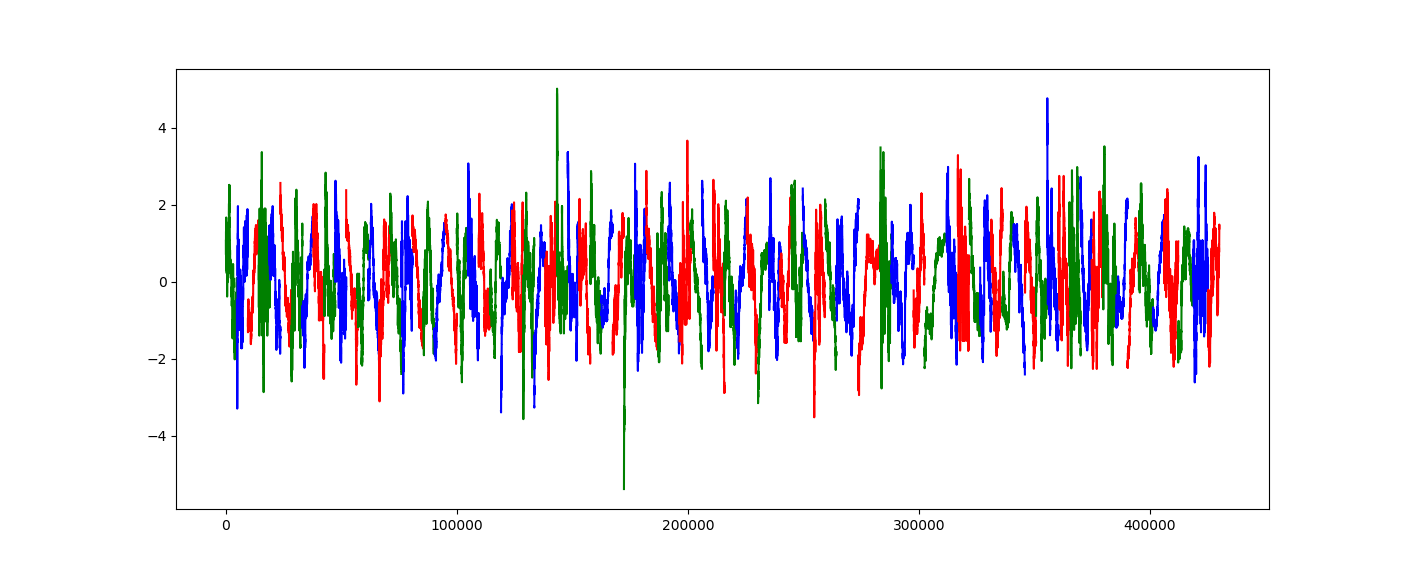
\includegraphics[scale = 0.4]{p8_2.png}
    \caption{MidPrice变化图(相邻相同颜色是同一天的数据)}
\end{figure}
\subsection{特征提取}
\paragraph{}进行归一化后,数据分布均匀度和相似度都提升了很多,但是,还有一个比较有趣的数据,那就是累计成交量了,数据如图8所示,从图中可以看出每日累计成交量是递增的,而且分布基本一致,并不能体现出与价格相关的特征,实际上,我们简单分析就可以知道,与成交量相比,更有意义的数据应该是成交增量,如果成交量大幅提高,很有可能就是卖方市场,成交价就会相应提高,相应的,如果成交量很小,成交价可能就会相应降低。这是比较符合我们所了解的经济学常识的。
\begin{figure}[!htbp]
    \centering
    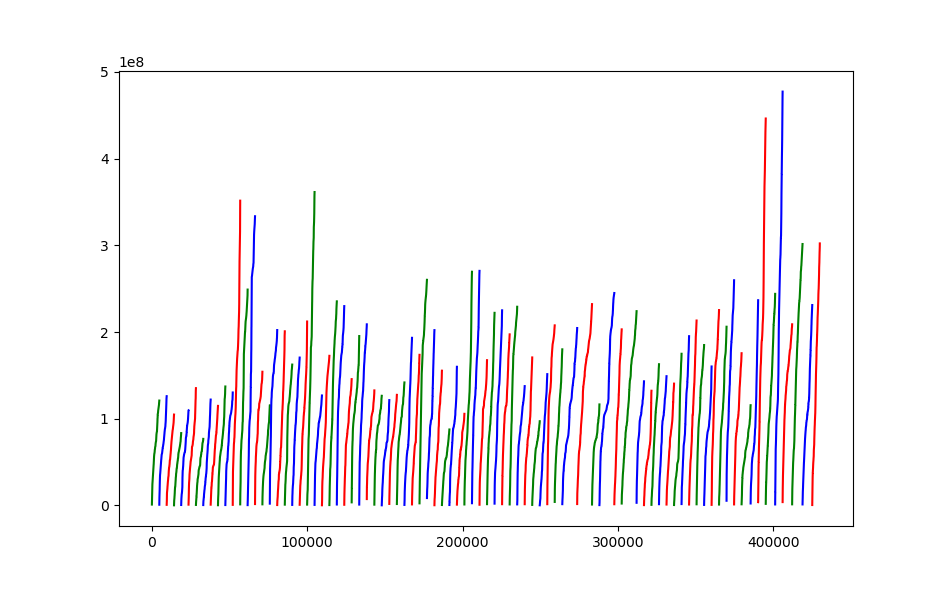
\includegraphics[scale = 0.5]{p9.png}
    \caption{Volume变化图(相邻相同颜色是同一天的数据)}
\end{figure}

\paragraph{}因此我们增加了一个新的feature,成交增量VolDiff.其分布归一化后如图9所示
\begin{figure}[!htbp]
    \centering
    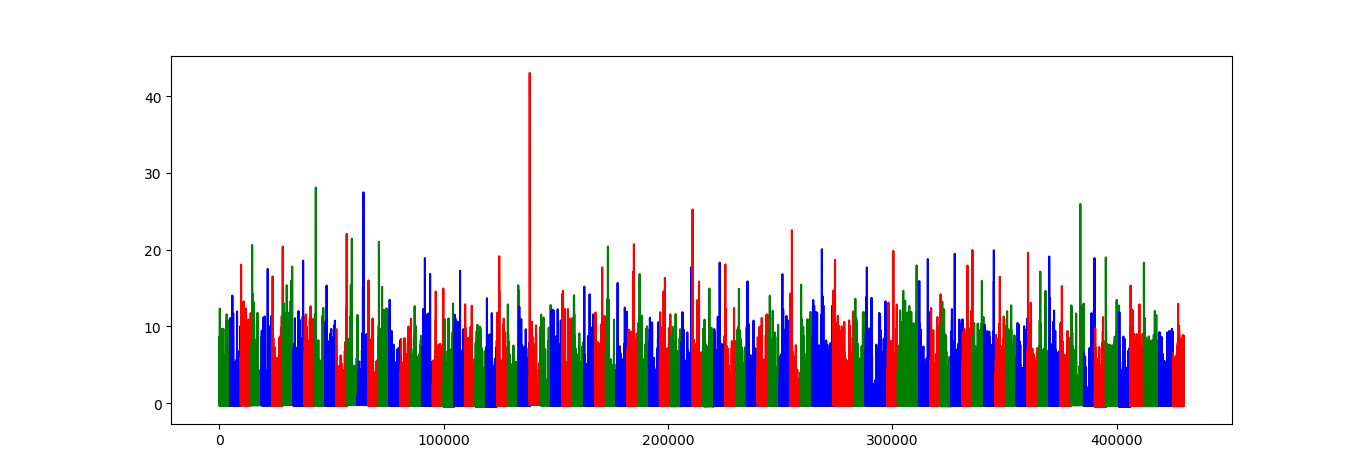
\includegraphics[scale = 0.4]{p9_2.png}
    \caption{VolDiff变化图(相邻相同颜色是同一天的数据)}
\end{figure}
由于图表为折线图,可能看的不是十分清楚,数据也是在均值0附近上下震荡.数据和成交价的相关性提高了很多。
\paragraph{}除了以上处理外,我们还清洗了无关的feature,例如时间和日期信息。
\subsection{结果分析}
经过对数据进行归一化处理,同时提取额外的特征VolDiff后,准确度有了大幅度提升,预测的loss从0.008下降到了0.0016附近

\section{思考与感悟}
\paragraph{}本次大作业,我了解到了股市交易的基本规则和分析方法。对于本次大作业,我们着重使用了LSTM模型对数据进行预测和分析。我了解到LSTM模型对于序列型的数据分析和预测效果非常好。我也对LSTM模型的数学原理以及代码实现有了一个比较深入的了解。
\paragraph{}同时我也了解到数据处理和特征提取的重要性。使用相同的模型,如果数据没有进行合适的预处理过程,模型将会难以训练,也不能得到正确的预测结果。在此次大作业过程中,模型数据没有进行以上介绍的预处理过程时,最终的预测结果非常差,与要求的精度差接近两个数量级,但是使用处理好的数据后,模型达到了要求的精度。
\paragraph{}在此次大作业过程中,我也真正体会到了机器学习的整个过程,从问题分析,模型选择与搭建,数据处理和分析,模型训练与调整等等。最深的体会莫过于机器学习十分耗费时间,每次调整都要仔细思考来提升效率。
\paragraph{}除了我对机器学习的体会外,这大作业还锻炼了我的很多方面,这次作业锻炼了我的耐心,也让我收获了很多课程上没有学到的很多知识。在数次调整都达不到要求时,我并没有选择放弃,而是继续努力,并且积极寻求同学的帮助,最终解决了问题。最后我想感谢我的队友和同学们,他们在我遇到困难时耐心指导,帮了我很多。感谢助教的辛苦工作,让我们能够顺利完成这次作业。

\begin{thebibliography}{3}
    \bibitem{1}https://colah.github.io/posts/2015-08-Understanding-LSTMs/
    \bibitem{2}https://blog.csdn.net/u012319493/article/details/52802302
    \bibitem{3}
    http://karpathy.github.io/2015/05/21/rnn-effectiveness/
    
\end{thebibliography}
\end{document}